\documentclass{exam}
\usepackage[utf8]{inputenc}
\usepackage[spanish,activeacute]{babel}
\usepackage{lmodern}
\usepackage[T1]{fontenc}
\usepackage{graphicx}
\usepackage{wrapfig}
\usepackage{eso-pic}
\usepackage{ragged2e}
\usepackage{float}
\usepackage{tabularx}
\usepackage{multicol,multirow}
\usepackage[margin=1in]{geometry}
\usepackage{amsmath,amssymb}
\usepackage{color}
\usepackage{fancyhdr}
\usepackage{lastpage}
\usepackage{titlesec}
\usepackage{sectsty}

\definecolor{azul}{RGB}{33,127,190}
\sectionfont{\color{azul}}
\subsectionfont{\color{azul}}

\fancypagestyle{plain}{
    \renewcommand{\headrulewidth}{0pt}%
    \fancyhf{}%
    \fancyfoot[R]{\footnotesize \color{azul}p{\'a}g. \thepage \hspace{1pt} de \pageref{LastPage}}%
}
\pagestyle{empty}
\pagestyle{fancy}
\fancyhf{}
\rfoot{
    {\footnotesize \color{azul}p{\'a}g. \thepage \hspace{1pt} de \pageref{LastPage}}
}

\newcommand{\makenonemptybox}[2]{%
    \par\nobreak\vspace{\ht\strutbox}\noindent
    \fbox{
        \parbox[c][\dimexpr#1-2\fboxsep][t]{\dimexpr\linewidth-2\fboxsep}{\hrule width \hsize height 0pt #2}
    }
    \par\vspace{\ht\strutbox}
}
\makeatother

\title{\huge\bfseries{\color{azul}Programaci\'on 2 - Certamen N$^{\circ}$ 3 }}
\author{\textbf{Eduardo Godoy.}}
\date{\em \today}

\begin{document}

\AddToShipoutPictureBG*{%
  \AtPageUpperLeft{\raisebox{-\height}{
\includegraphics[scale=0.95]{img/header.png}}}}

%% --- CABECERA --- %%

\maketitle

\begin{multicols}{2}
    \begin{flushleft}
        \textbf{Nombre:} \\
        \vspace*{2mm}
        \textbf{Rut:}
    \end{flushleft}
    \begin{center}
        \begin{table}[H]
        \begin{tabular}{p{4cm}|p{3cm}|}
        \cline{2-2}
            ~ & {\em {\scriptsize Puntaje}} \\ & ~ \\
            ~ & \textbf{Nota} \\ & ~ \\
        \cline{2-2}
        \end{tabular}
        \end{table}
    \end{center}
\end{multicols}

%% --- INSTRUCCIONES --- %%

\vspace*{-7mm}
\noindent
\textbf{Resultados de aprendizaje a evaluar:}
\begin{enumerate}
  \item Conceptos generales de Orientada a Objetos.
  \item Utilizaci\'on de Lenguaje Java y sus caracter\'isticas pricipales para resolver problemas.
  \item Diseño e implementaci\'on de interfaces de usuario.
  \item Implementaci\'on y explotaci\'on de fuentes de persistencia de informaci\'on.
\end{enumerate}
\vspace{5mm}
\noindent
\textbf{Instrucciones:}
\begin{itemize}
  \item[-] El puntaje m\'aximo del certamen es 100\%, siendo el 60\% el m\'inimo requerido para aprobar.
  %\item[-] Responda cada pregunta en la hoja indicada, agregando su nombre. Si no responde alguna pregunta, debe entregar la hoja con su nombre e indicar que \textbf{no responde}.
  \item[-] El certamen es \underline{\textbf{resuelto en grupos de dos personas}}.
\end{itemize}

\vspace{5mm}
\noindent
\textbf{Contenido:}.

\vspace{2mm}
\noindent
\begin{table}[H]
{\normalsize
\begin{tabular}{|p{9.5cm}|p{3.3cm}|p{3.3cm}|}
\hline
    \multicolumn{1}{|c}{\textbf{Tema}} &
    \multicolumn{1}{|c}{\textbf{Puntaje total}} &
    \multicolumn{1}{|c|}{\textbf{Puntaje obtenido}} \\
\hline
    Java aplicaci\'on de caracter\'isticas del lenguaje para solucionar un problema  &
    \multicolumn{1}{|c|}{\textbf{30 puntos}} & \\
\hline
    Java Swing y Manejo de Archivos &
    \multicolumn{1}{|c|}{\textbf{30 puntos}} & \\
\hline
    Evaluaci\'on de conceptos de Orientaci\'on a Objetos y aplicaci\'on de estos a la resoluci\'on del problema&
    \multicolumn{1}{|c|}{\textbf{40 puntos}} & \\
\hline
\end{tabular}}
\end{table}

\vspace{-2mm}
\noindent
\textbf{Puntaje total:} 100 puntos \textbf{Exigencia:} 60\% \textbf{Tiempo:} 48 horas.

%% --- INICIO CERTAMEN --- %%
\newpage
\noindent
\section{\textbf{Java Threads ( 30 pts)}}
\noindent

       \item Un videojuego tiene \textbf{Personajes} los cuales se enfrentan en una batalla definida por turnos. Cada personaje tiene un \emph{nombre} (String) y un
       \emph{nivel propio de energ\'ia} (int). Adem\'as poseen la capacidad de  \emph{alimentarse} (m\'etodo), que recibe por par\'ametro
       una cantidad de energ\'ia (int) con el que incrementa el \emph{nivel propio de energ\'ia}. Los personajes pueden ser:
       \begin{itemize}
         \item \textbf{Guerreros}:
         \begin{itemize}
           \item Tienen adem\'as un \emph{arma} (String). La cual posee 3 tipos de ataques:
           \begin{enumerate}
             \item[-] Golpe directo: Da\~na al oponente restandole 20 puntos de energia.
             \item[-] Giro letal: Da\~na al oponente de forma reiterada restandole 30 puntos de energia.
             \item[-] Super arma: El arma triplica su tama\~no da\~nando al oponente y restandole 70 puntos de energia. A su vez el guerrero se resta puntos de vida equivalentes al 30\% del da\~no realizado.
             \item[-] Pierde turno: El oponente logra eludir el ataque del guerrero.
           \end{enumerate}
           \item Cada uno de los ataques anteriores se ejecutan  de forma aleatoria y uno por turno, siendo el 0 Golpe directo, 1 Giro letal, 2 Super arma, 3 Pierde turno.
           \item Estos ataques se ejecutan mediante la invocaci\'on del m\'etodo combatir().
           \item Al momento de la instanciaci\'on del Mago, este recibe su  \emph{nombre} y \emph{arma}.
           \item Los guerreros son siempre creados con un \emph{nivel propio de energ\'ia} igual a 150.
          \item Al momento de la instanciaci\'on reciben su \emph{nombre},  \emph{arma} y \emph{nivel propio de energ\'ia} inicial.
        \end{itemize}

         \item \textbf{Magos}:

           \begin{itemize}
           \item Tienen adem\'as un \emph{hechizo} (String).  El cual posee 3 niveles de daño definidos a continuaci\'on:
           \begin{itemize}
             \item[-] Llamarada: El mago envia una flama  da\~nando al oponente y restandole 20 puntos de energia.
             \item[-] Insendio: Insinera al oponete y su entorno da\~nandolo y restandole 35 puntos de energia. Adem\'as se emite una jugada adicional aleatoria entre 0 y 1 siendo 0 no afecta con mas daño y 1 afecta con 5 puntos m\'as al daño final.
             \item[-] Explosi\'on: El mago emite una explosi\'on  da\~nando al oponente restandole 60 puntos de energia.  Al ejecutar esta habilidad el mago puede recuperar  energia ejecutando el m\'etodo alimentarse() por el 50\% del da\~no realizado al oponente.
             \item[-] Pierde turno: El mago falla la ejecuci\'on del ataque.
           \end{itemize}
             \item Cada uno de los ataques anteriores se ejecutan  de forma aleatoria y uno por turno, siendo el 0 Llamarada, 1 Insendio, 2 Explosi\'on, 3 Pierde turno.
             \item Estos ataques se ejecutan mediante la invocaci\'on del m\'etodo encantar().
             \item Al momento de la instanciaci\'on del Mago, este recibe su  \emph{nombre} y \emph{hechizo}.
             \item Los magos son siempre creados con un \emph{nivel propio de energ\'ia} igual a 100.
             \item Poseen el m\'etodo \emph{encantar} que disminuye en 2 unidades el \emph{nivel propio de energ\'ia} cada ves que se ejecuta un ataque exitos.
           \end{itemize}
     \item El combate termina cuando la energ\'ia      de uno de los dos personajes sea menor o igual a 0.
     \item El estado del combate se debe visualizar por consola mediante el siguiente formato: \emph{Personaje;tipo de ataque;daño realizado}.
     \item La generalizaci\'on de las clases se muestra en la figura~\ref{fig-modelo}.
     \begin{figure}[htbp!]
       \begin{center}
         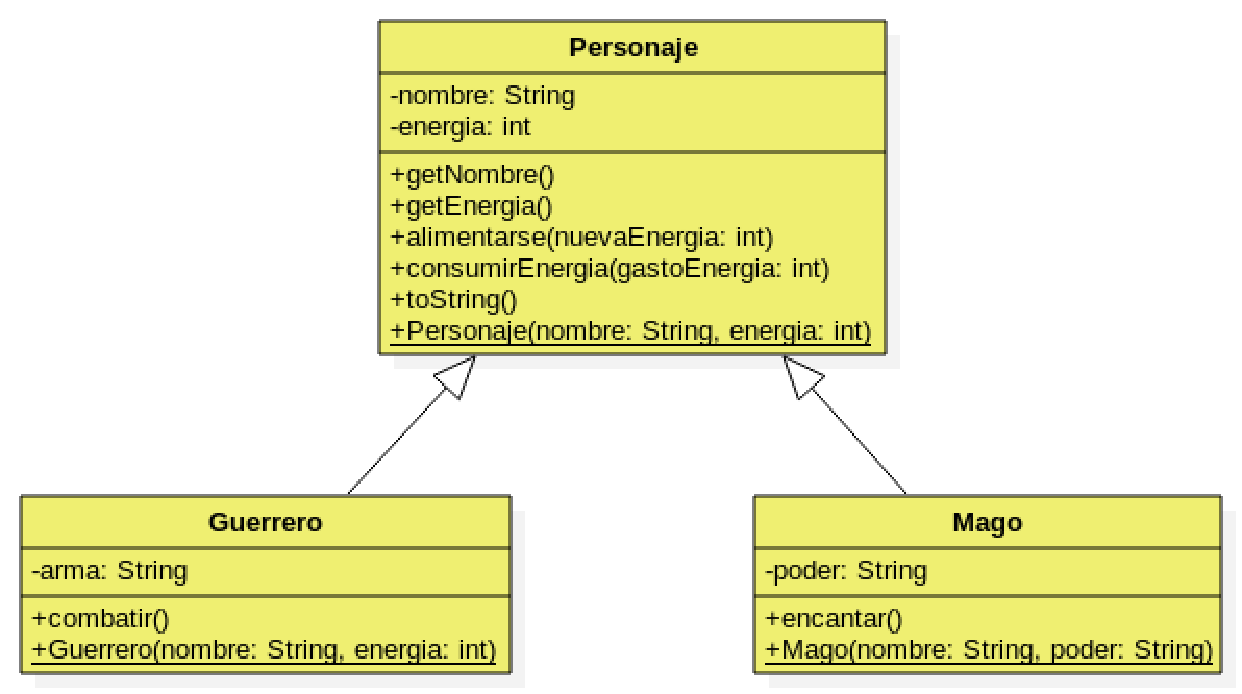
\includegraphics[width=10cm]{img/modelo.pdf}
         \caption{{\small Diagrama de clases}}\label{fig-modelo}
       \end{center}
     \end{figure}
     \item Desarrolle las clases e interface mostradas en el modelo.
     \item implemente los Java Threads asociados al Mago y Guerrero, los cuales simularan el compate  permitan ejecutar los ataques de cada uno.
     \item Implemente la clase que maneje los estados de energía de los pesonajes y permita ejecutar sus ataques de aleatorios segun lo indicado anteriormente.
     \item implemente una clase que escriba en dos archivos lo siguiente:
     \begin{itemize}
       \item[-] El primero llamado ataque.csv debe agregar por cada turno un registro con el da\~no realizado segun el siguiente formato: \emph{Personaje;tipo de ataque;daño realizado}.
       \item[-] El segundo llamado danio.csv debe agregar por cada turno un registro con el da\~no recibido seg\'un el siguiente formato: \emph{Personaje;da\~no realizado}.
     \end{itemize}
           \item Implementar la clase que debe utilizar los m\'etodos para \emph{combatir} y \emph{alimentarse}.
      \item La clase principal que permita instanciar personajes de tipo guerreros y magos. Luuego iniciar la batalla.
       \end{itemize}


         \begin{table}[!ht]
            {\scriptsize
             \begin{center}
                  \begin{tabular}{|p{1.5cm}|p{5.5cm}|p{5.5cm}|p{3cm}|}\hline
                     \multicolumn{4}{|c|}{\textbf{\textquestiondown C\'omo ser\'e evaluado este Control?} } \\ \hline
                     \multicolumn{1}{|c|}{\textbf{T\'opico}} &
                     \multicolumn{1}{c|}{\textbf{Logrado}} &
                     \multicolumn{1}{c|}{\textbf{Medianamente logrado}} &
                     \multicolumn{1}{c|}{\textbf{No logrado}} \\ \hline
                     T\'opico 1 - Java Interface . &
                     \emph{5pts} Crea las Interface  Persona  con sus  m\'etodos	requeridos. &
                     \emph{2pts} Crea Interface con algunos   m\'etodos	requeridos en el. Crea m\'etodos o Atributos en otras clases no indicadas en el problema. &
                     \emph{  0pts} No crea clases requeridas. \\ \hline


                     T\'opico 1-a - Clase Guerrero  &
                     \emph{5pts} Define e implementa la Clase Guerrero con sus  m\'etodos relacionados &
                     \emph{2pts} Define e implementa m\'etodo acercandose parcialmente a la salida esperada. &
                     \emph{ 0pts} No define m\'etodo o definido pero no cumple con lo m\'inimo esperado.\\ \hline

                     T\'opico 1-b - Clase Mago &
                     \emph{5pts} Define e implementa la Clase Mago con sus  m\'etodos relacionados. &
                     \emph{2pts} Define e implementa m\'etodo acercandose parcialmente a la salida esperada. &
                     \emph{ 0pts} No define m\'etodo o definido pero no cumple con lo m\'inimo esperado. \\ \hline

                     T\'opico 2 - ThreadMago&
                     \emph{5pts} Define e implementa la clase Thread para simular el ataque de Mago  con sus m\'etodos y  atributos requeridos.&
                     \emph{2pts} Define e implementa la clase acercandose parcialmente a la salida esperada.  &
                     \emph{ 0pts} No define clase o definida pero no cumple con lo m\'inimo esperado. \\ \hline

                     T\'opico 3 - ThreadGuerrero&
                     \emph{5pts} Define e implementa la clase Thread para simular el ataque de Guerrero  con sus m\'etodos y  atributos requeridos.&
                     \emph{2pts} Define e implementa la clase acercandose parcialmente a la salida esperada.  &
                     \emph{ 0pts} No define clase o definida pero no cumple con lo m\'inimo esperado. \\ \hline

                     T\'opico 4 - Clase Combate &
                     \emph{5pts} Define e implementa la clase de que permite coordinar el combate de los Personajes simulaci\'on del combate con sus m\'etodo main incluidos.&
                     \emph{2pts} Define e implementa clase y m\'etodo acercandose parcialmente a la salida esperada.  &
                     \emph{ 0pts} No define m\'etodo o definido pero no cumple con lo m\'inimo esperado. \\ \hline

                     T\'opico 5 - Clase Inicializadora &
                     \emph{5pts} Define e implementa la clase de control que permite iniciar el proceso de simulaci\'on del combate con sus m\'etodo main incluido.&
                     \emph{2pts} Define e implementa clase y m\'etodo acercandose parcialmente a la salida esperada.  &
                     \emph{ 0pts} No define m\'etodo o definido pero no cumple con lo m\'inimo esperado. \\ \hline

                     Paradigma Orientaci\'on a Objetos  &
                     \emph{5pts} Resuelve el problema utilizando OO y patrones de dise\~nos presentados en clase. &
                     \emph{3pts} Utiliza parte del POO y  patrones de dise\~no para resolver el problema. &
                     \emph{0pts} No utiliza el POO para dar soluci\'on al problema.\\ \hline
                     Total m\'aximo puntaje pregunta 2 &
                     \emph{40pts} &
                     \emph{17pts} &
                     \emph{  0pts} \\ \hline
                 \end{tabular}
             \end{center}}
          \end{table}
\end{itemize}


\section{\textbf{Java Swing y Archivos (30 pts)}}
\noindent



    		\item  Una vez finalizado el combate y utilizando los archivos generados a partir del resultado de la pregunta 1, realizar lo siguiente:
          \begin{itemize}
            \item Generar una interfaz con Java Swing que permita visualizar:
              \begin{enumerate}
                \item En su parte superior: Dos botones con los nombre respectivos de cada personaje.
                \item En su parte inferior: Dos Tabla de Datos.
                \item Al presionar un boton, \'este recuperar\'a los registros desde el archivos asociados al personaje que referencia el boton.
                \item En la tabla de datos izquierda se debe desplegar el da\n~o realizado y en la derecha el daño recibido.
                \item En el desarrollo de esta interfaz se requiere implementar los patrones de diseño vistos en clases.
                \item incluir buenas practicas de programaci\'on.
              \end{enumerate}
          \end{itemize}

    	\begin{table}[!ht]
           {\scriptsize
            \begin{center}
                 \begin{tabular}{|p{3.5cm}|p{3.5cm}|p{3.5cm}|p{3.5cm}|}\hline
                    \multicolumn{4}{|c|}{\textbf{\textquestiondown C\'omo ser\'e evaluado en la pregunta 2?} } \\ \hline
                    \multicolumn{1}{|c|}{\textbf{T\'opico}} &
                    \multicolumn{1}{c|}{\textbf{Logrado}} &
                    \multicolumn{1}{c|}{\textbf{Medianamente logrado}} &
                    \multicolumn{1}{c|}{\textbf{No logrado}} \\ \hline
                    Manipulaci\'on de archivo. &
                    \emph{5pts} Lee correctamente los archivos, los mapea a entidad  y crea ArrayList. &
                    \emph{3pts} Realiza dos de las tres acciones del punto anterior. &
                    \emph{ 0pts} No realiza la acciones del punto anterior. \\ \hline
                    Diseño e implementación de interfaz. &
                    \emph{15pts} Crea la interfaz de forma correcta y con los componentes requeridos. &
                    \emph{7pts} Crea la interfaz de forma correcta e  implementa algunos componentes requeridos. &
                    \emph{ 0pts} No crea interfaz. \\ \hline
                    Integración Interfaz con contenido de archivos &
                    \emph{15pts} Asocia acciones a botones y despliega registros en tablas según lo requerido en el problema. &
                    \emph{7pts} Crea la clase entidad para Movie o la Rating (no ambas). &
                    \emph{0pts} No crea las clases entidad. \\ \hline
                    Paradigma Orientaci\'on a Objetos  &
                    \emph{5pts} Implementa la solución según patrones de dise\n~o y programas vistos en clases. &
                    \emph{2pts} Implementa la solución sin patrones de diseño. &
                    \emph{0pts} No se implementa seg\'un lo indicado. \\ \hline

                    Total m\'aximo puntaje pregunta 2 &
                    \emph{40pts} &
                    \emph{18pts} &
                    \emph{0pts} \\ \hline
                \end{tabular}
            \end{center}}
         \end{table}

         \newpage
         \noindent
         \section{\textbf{Interrogaci\'on (40 pts)}}
 \noindent
           \emph Interrogaci\'on individual sobre codificación y aplicación de conceptos dentro de la soluci\'on entregada.
            \begin{enumerate}
              \item Pregunta de manejo de conceptos aplicados a la soluci\'on implementada.
              \item Pregunta de codificación 1.
              \item Pregunta de codificación 2.
            \end{enumerate}
         	\end{enumerate}

          \begin{table}[!ht]
               {\scriptsize
                \begin{center}
                     \begin{tabular}{|p{3.5cm}|p{3.5cm}|p{3.5cm}|p{3.5cm}|}\hline
                        \multicolumn{4}{|c|}{\textbf{\textquestiondown C\'omo ser\'e evaluado en la pregunta 3?} } \\ \hline
                        \multicolumn{1}{|c|}{\textbf{T\'opico}} &
                        \multicolumn{1}{c|}{\textbf{Logrado}} &
                        \multicolumn{1}{c|}{\textbf{Medianamente logrado}} &
                        \multicolumn{1}{c|}{\textbf{No logrado}} \\ \hline
                        Pregunta de manejo de Conceptos aplicados a la soluci\'on. &
                        \emph{15pts} Responde de forma correcta  seg\'un lo esperado. &
                        \emph{8pts} Responde de forma inconpleta o con apoyo del profesor. &
                        \emph{0pts} No responde seg\'un lo esperado. \\ \hline
                        Pregunta de códificación 1. &
                        \emph{15pts} Responde de forma correcta  seg\'un lo esperado. &
                        \emph{8pts} Responde de forma inconpleta o con apoyo del profesor. &
                        \emph{ 0pts} No responde seg\'un lo esperado. \\ \hline
                        Pregunta de códificación 1. &
                        \emph{10pts} Responde de forma correcta  seg\'un lo esperado. &
                        \emph{5pts} Responde de forma inconpleta o con apoyo del profesor. &
                        \emph{0pts} No responde seg\'un lo esperado. \\ \hline

                        Total m\'aximo puntaje pregunta 2 &
                        \emph{40pts} &
                        \emph{20pts} &
                        \emph{0pts} \\ \hline
                    \end{tabular}
                \end{center}}
             \end{table}

          \textbf{Condiciones de entrega:}
          \begin{itemize}
              \item[-] \textbf{Debe compilar}.
              \item[-] Enviar al correo eduardo.gl@gmail.com con el proyecto comprimido, eliminado de ante mano los archivos .class.
              \item[-] Debe llevar como asunto Certamen 2 y  un comprimido con formato {Certamen\_2\_.zip} adjuntado.
              \item[-] Se debe incluir dentro del comprimido un archivo de tipo .txt  que contenga nombre apellido y rut de ambos integrantes del grupo.
        			\item[-] El no cumplimiento del formato ser\'a penalizado con 10 punto de descuento.
              \item[-] Entrega Sabado 2 de noviembre antes de las 23:59 am. Subir hasta la hora indicada en el certamen.
        			\item[-] El no cumplimiento con la hora de entrega, ser\'a penalizado con 2 punto de descuento por cada minuto de retraso.
              \item[-] Si bien el trabajo colaborativo esta permitido, la presunci\'on o evidencia de copia entre dos o mas grupos ser\'a penalizada con 30 de descuento  de la nota final para cada uno.
          \end{itemize}

\end{questions}

\end{document}
